\section{What is Aging?}

\subsection{Definition and Hallmarks}

\begin{frame}[c]{Aging}
    \large

    \begin{block}{Definition \cite{sen2016epigenetic}}
        Aging is characterized by progressive decline in tissue and organ
        function and increased risk of mortality.
    \end{block}
    \pause
    But how can we measure it?
    \pnote{
        If someone remembers: ask me what aging is \\
        biologically, not enough time now
    }
\end{frame}


\begin{frame}[c]{Hallmarks of Aging: Measuring biological Age}
    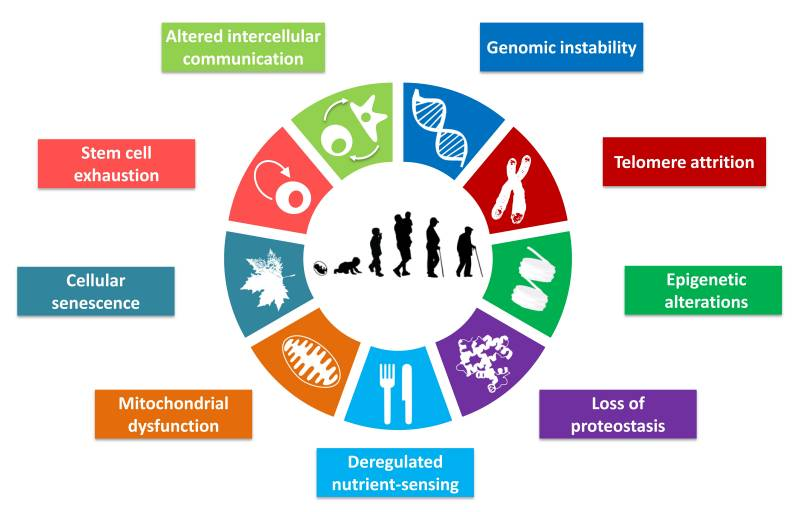
\includegraphics[width=\textwidth]{hallmarks_aging} \\
    Source: \cite{lopez2013hallmarks}
    \pnote{
        Groundbreaking paper, one of the most-cited \\
        Aging: accumulating damage to hallmark \\
        \par
        One hallmark also affects and damages others \\
        Classified as Primary (causes), Antagonistic \\
        (responses), Integrative (phenotype) \\
        Unclear if actually the case \\
    }
\end{frame}

\subsection{Problematic: Many Unknowns}

\begin{frame}[c]{Problem: Many Theories}
    \large
    \begin{itemize}[<+(1)->]
        \item Everything is interlinked
        \item Very hard to distinguish cause and effect
        \item At least one Theory for every Hallmark
        \item Every prestigious lab has its own Theory
        \item A lot of speculation on most sides
        \item Unclear if we can already see the full picture
        \item More research is needed
    \end{itemize}
    \pnote{Unclear if we have all the puzzle pieces \\ to solve it}
\end{frame}

\addtocounter{framenumber}{1}
\begin{frame}[standout]
    Disclaimer: Any misrepresentation or mistaken interpretation is due to my shortcomings
\end{frame}
